%(BEGIN_QUESTION)
% Copyright 2011, Tony R. Kuphaldt, released under the Creative Commons Attribution License (v 1.0)
% This means you may do almost anything with this work of mine, so long as you give me proper credit

Undersøk ``Siemens/Moore 353 program for pulse-width modulation'' i Instrumentation Reference, som viser et funksjonsblokkprogram der 353-regulatoren får PWM-utgang (modulert av/på) i stedet for analog 4--20 mA-utgang. Svar deretter på spørsmålene:

\vskip 10pt

Identifiser hvilke funksjonsblokker som er koblet likt som i standard Factory Configured Option 101-program, og hvilke som avviker.

\vskip 10pt

Forklar hvorfor noen ønsker en reguleringssløyfe med PWM-utgang i stedet for analog 4--20 mA-utgang.

\vskip 10pt

Forklar hvordan denne analoge kretsen lager et PWM-utgangssignal fra et sagtannsignal og en DC-referanse, og hvordan funksjonen etterlignes av funksjonsblokkprogrammet i Siemens 353-regulatoren:

$$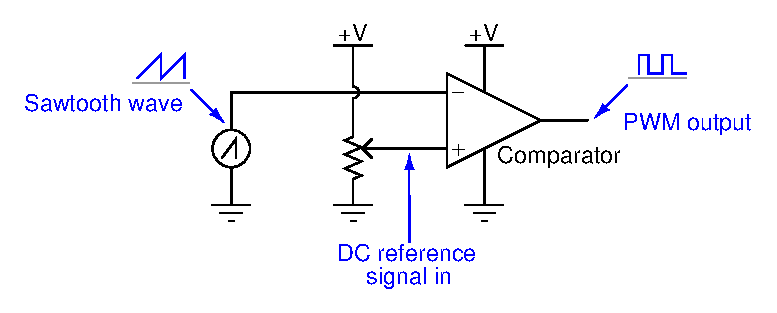
\includegraphics[width=15.5cm]{i00356x01.eps}$$



\vskip 20pt \vbox{\hrule \hbox{\strut \vrule{} {\bf Forslag til sokratisk diskusjon} \vrule} \hrule}

\begin{itemize}
\item{} Beskriv trinnene som trengs for å redigere FCO 101-programmet slik at det ligner dette programmet, ved hjelp av frontpanelknapper og display.
\item{} Hvilken vei må du flytte glideren på potensiometeret i den analoge kretsen for å øke duty cycle i PWM-utgangen?
\item{} Hva blir effekten hvis +V-tilkoblingen til potensiometeret får brudd?
\item{} Hva blir effekten hvis jordtilkoblingen til potensiometeret får brudd?
\item{} Hva blir effekten hvis sagtanngeneratoren feiler og gir 0 volt ut?
\item{} Hva blir effekten hvis +V-tilkoblingen til komparatoren får brudd?
\item{} Skisser en ``interposing''-krets som kan ta opamp-utgangen og forsterke den slik at den kan drive PWM-effekt til et stort elektrisk varmeelement (for eksempel 240 VAC).
\end{itemize}

\underbar{file i00356}
%(END_QUESTION)





%(BEGIN_ANSWER)


%(END_ANSWER)





%(BEGIN_NOTES)

AIN1-, SETPT-, PID- og A/M-funksjonsblokkene er alle del av standard FCO 101-program. Alle andre blokker er lagt til for å få denne PWM-funksjonen.

\vskip 10pt

Et regulatorprogram med PWM-utgang er nyttig når regulatoren styrer en diskret sluttkontrollenhet, som et elektrisk varmeelement (av/på) eller en magnetventil.

\vskip 10pt

Komparatoren sammenligner sagtannspenningen med DC-referansen satt av potensiometeret. Når DC-referansespenningen er høyere enn sagtannspenningen, går komparatorutgangen høy. Når sagtannspenningen stiger og faller, veksler komparatorutgangen mellom høy og lav og danner et pulstog. Når DC-referansen økes, blir tiden i ``høy''-tilstand lengre og tiden i ``lav''-tilstand kortere, og duty cycle øker.

%INDEX% Reading assignment: Siemens model 353 controller program for PWM control

%(END_NOTES)
